%!TeX root=../viewsbodytop.tex
\addchap{The Fascinating Problem of Uncle Meleager's Will}

\lettrine[lines=4,ante=‘]{Y}{ou} look a little worried, Bunter,' said his lordship kindly to his manservant. »Is there anything I can do?«

\zz
The valet's face brightened as he released his employer's grey trousers from the press.

»Perhaps your lordship could be so good as to think,« he said hopefully, »of a word in seven letters with S in the middle, meaning two.«

»Also,« suggested Lord~Peter thoughtlessly.

»I beg your lordship's pardon. T-w-o. And seven letters.«

»Nonsense!« said Lord~Peter. »How about that bath?«

»It should be just about ready, my lord.«

Lord~Peter Wimsey swung his mauve silk legs lightly over the edge of the bed and stretched appreciatively. It was a beautiful June that year. Through the open door he saw the delicate coils of steam wreathing across a shaft of yellow sunlight. Every step he took into the bathroom was a conscious act of enjoyment. In a husky light tenor he carolled a few bars of »Maman, dites-moi.« Then a thought struck him, and he turned back.

»Bunter!«

»My lord?«

»No bacon this morning. Quite the wrong smell.«

»I was thinking of buttered eggs, my lord.«

»Excellent. Like primroses. The Beaconsfield touch,« said his lordship approvingly.

His song died into a rapturous crooning as he settled into the verbena-scented water. His eyes roamed vaguely over the pale blue-and-white tiles of the bathroom walls.

Mr~Bunter had retired to the kitchen to put the coffee on the stove when the bell rang. Surprised, he hastened back to the bedroom. It was empty. With increased surprise, he realised that it must have been the bathroom bell. The words »heart-attack« formed swiftly in his mind, to be displaced by the still more alarming thought, »No soap.« He opened the door almost nervously.

»Did you ring, my lord?« he demanded of Lord~Peter's head, alone visible.

»Yes,« said his lordship abruptly; »Ambsace.«

»I beg your lordship's pardon?«

»Ambsace. Word of seven letters. Meaning two. With S in the middle. Two aces. Ambsace.«

Bunter's expression became beatified.

»Undoubtedly correct,« he said, pulling a small sheet of paper from his pocket, and entering the word upon it in pencil. »I am extremely obliged to your lordship. In that case the »indifferent cook in six letters ending with red« must be Alfred.«

Lord~Peter waved a dismissive hand.

\divider
On re-entering his bedroom, Lord~Peter was astonished to see his sister Mary seated in his own particular chair and consuming his buttered eggs. He greeted her with a friendly acerbity, demanding why she should look him up at that unearthly hour.

»I'm riding with Freddy Arbuthnot,« said her ladyship, »as you might see by my legs, if you were really as big a Sherlock as you make out.«

»Riding,« replied her brother; »I had already deduced, though I admit that Freddy's name was not writ large, to my before-breakfast eye, upon the knees of your breeches. But why this visit?«

»Well, because you were on the way,« said Lady~Mary, »and I'm booked up all day, and I want you to come and dine at the Soviet Club with me to-night.«

»Good God, Mary, why? You know I hate the place. Cooking's beastly, the men don't shave, and the conversation gets my goat. Besides, last time I went there, your friend Goyles plugged me in the shoulder. I thought you'd chucked the Soviet Club.«

»It isn't me. It's Hannah Marryat.«

»What, the intense young woman with the badly bobbed hair and the brogues?«

»Well, she's never been able to afford a good hairdresser. That's just what I want your help about.«

»My dear child, I can't cut her hair for her. Bunter might. He can do most things.«

»Silly. No. But she's got—that is, she used to have—an uncle, the very rich, curmudgeony sort, you know, who never gave anyone a penny. Well, he's dead, and they can't find his will.«

»Perhaps he didn't make one.«

»Oh, yes, he did. He wrote and told her so. But the nasty old thing hid it, and it can't be found.«

»Is the will in her favour?«

»Yes.«

»Who's the next-of-kin?«

»She and her mother are the only members of the family left.«

»Well, then, she's only got to sit tight and she'll get the goods.«

»No—because the horrid old man left two wills, and, if she can't find the latest one, they'll prove the first one. He explained that to her carefully.«

»Oh, I see. H'm. By the way, I thought the young woman was a Socialist.«

»Oh, she is. Terrifically so. One really can't help admiring her. She has done some wonderful work\longdash«

»Yes, I dare say. But in that case I don't see why she need be so keen on getting uncle's dollars.«

Mary began to chuckle.

»Ah! but that's where Uncle Meleager\longdash«

»Uncle what?«

»Meleager. That's his name. Meleager Finch.«

»Oh!«

»Yes—well, that's where he's been so clever. Unless she finds the new will, the old will comes into force and hands over every penny of the money to the funds of the Primrose League.«

Lord~Peter gave a little yelp of joy.

»Good for Uncle Meleager! But, look here, Polly, I'm a Tory, if anything. I'm certainly not a Red. Why should I help to snatch the good gold from the Primrose Leaguers and hand it over to the Third International? Uncle Meleager's a sport. I take to Uncle Meleager.«

»Oh, but Peter, I really don't think she'll do that with it. Not at present, anyway. They're awfully poor, and her mother ought to have some frightfully difficult operation or something, and go and live abroad, so it really is ever so important they should get the money. And perhaps Hannah wouldn't be quite so Red if she'd ever had a bean of her own. Besides, you could make it a condition of helping her that she should go and get properly shingled at Bresil's.«

»You are a very cynically-minded person,« said his lordship. »However, it would be fun to have a go at Uncle M\@. Was he obliging enough to give any clues for finding the will?«

»He wrote a funny sort of letter, which we can't make head or tail of. Come to the club to-night and she'll show it to you.«

»Right-ho! Seven o'clock do? And we could go on and see a show afterwards. Do you mind clearing out now? I'm going to get dressed.«

\divider
Amid a deafening babble of voices in a low-pitched cellar, the Soviet Club meets and dines. Ethics and sociology, the latest vortices of the Whirligig school of verse, combine with the smoke of countless cigarettes to produce an inspissated atmosphere, through which flat, angular mural paintings dimly lower upon the revellers. There is painfully little room for the elbows, or indeed for any part of one's body. Lord~Peter—his feet curled under his chair to avoid the stray kicks of the heavy brogues opposite him—was acutely conscious of an unbecoming attitude and an overheated feeling about the head. He found it difficult to get any response from Hannah Marryat. Under her heavy, ill-cut fringe her dark eyes gloomed sombrely at him. At the same time he received a strong impression of something enormously vital. He had a sudden fancy that if she were set free from self-defensiveness and the importance of being earnest, she would exhibit unexpected powers of enjoyment. He was interested, but oppressed. Mary, to his great relief, suggested that they should have their coffee upstairs.

They found a quiet corner with comfortable chairs.

»Well, now,« said Mary encouragingly.

»Of course you understand,« said Miss Marryat mournfully, »that if it were not for the monstrous injustice of Uncle Meleager's other will, and mother being so ill, I shouldn't take any steps. But when there is \textsterling 250,000, and the prospect of doing real good with it\longdash«

»Naturally,« said Lord~Peter, »it isn't the money you care about, as the dear old bromide says, it's the principle of the thing. Right you are! Now supposin' we have a look at Uncle Meleager's letter.«

Miss Marryat rummaged in a very large hand-bag and passed the paper over.

This was Uncle Meleager's letter, dated from Siena twelve months previously.

\makeatletter
\@ifclasswith{scrbook}{a5paper}
{%

}{%
	\enlargethispage{\baselineskip}
}
\makeatother

% \begin{quotation}
% \textsc{My dear Hannah,}—When I die—which I propose to do at my own convenience and not at that of my family—you will at last discover my monetary worth. It is, of course, considerably less than you had hoped, and quite fails, I assure you, adequately to represent my actual worth in the eyes of the discerning. I made my will yesterday, leaving the entire sum, such as it is, to the Primrose League—a body quite as fatuous as any other in our preposterous state, but which has the advantage of being peculiarly obnoxious to yourself. This will will be found in the safe in the library.

% I am not, however, unmindful of the fact that your mother is my sister, and you and she my only surviving relatives. I shall accordingly amuse myself by drawing up to-day a second will, superseding the other and leaving the money to you.

% I have always held that woman is a frivolous animal. A woman who pretends to be serious is wasting her time and spoiling her appearance. I consider that you have wasted your time to a really shocking extent. Accordingly, I intend to conceal this will, and that in such a manner that you will certainly never find it unless by the exercise of a sustained frivolity.

% I hope you will contrive to be frivolous enough to become the heiress of your affectionate
% \begin{flushright}
% »\textsc{Uncle Meleager.}«
% \end{flushright}
% \end{quotation}


\begin{mail}{}{My dear Hannah,}
	When I die—which I propose to do at my own convenience and not at that of my family—you will at last discover my monetary worth. It is, of course, considerably less than you had hoped, and quite fails, I assure you, adequately to represent my actual worth in the eyes of the discerning. I made my will yesterday, leaving the entire sum, such as it is, to the Primrose League—a body quite as fatuous as any other in our preposterous state, but which has the advantage of being peculiarly obnoxious to yourself. This will will be found in the safe in the library.

I am not, however, unmindful of the fact that your mother is my sister, and you and she my only surviving relatives. I shall accordingly amuse myself by drawing up to-day a second will, superseding the other and leaving the money to you.

I have always held that woman is a frivolous animal. A woman who pretends to be serious is wasting her time and spoiling her appearance. I consider that you have wasted your time to a really shocking extent. Accordingly, I intend to conceal this will, and that in such a manner that you will certainly never find it unless by the exercise of a sustained frivolity.
	
	\closeletter[I hope you will contrive to be frivolous enough to become the heiress of your affectionate]{Uncle Meleager.}
\end{mail}

»Couldn't we use that letter as proof of the testator's intention, and fight the will?« asked Mary anxiously.

»'Fraid not,« said Lord~Peter. »You see, there's no evidence here that the will was ever actually drawn up. Though I suppose we could find the witnesses.«

»We've tried,« said Miss Marryat, »but, as you see, Uncle Meleager was travelling abroad at the time, and he probably got some obscure people in some obscure Italian town to witness it for him. We advertised, but got no answer.«

»H'm. Uncle Meleager doesn't seem to have left things to chance. And, anyhow, wills are queer things, and so are the probate and divorce wallahs. Obviously the thing to do is to find the other will. Did the clues he speaks of turn up among his papers?«

»We hunted through everything. And, of course, we had the whole house searched from top to bottom for the will. But it was quite useless.«

»You've not destroyed anything, of course. Who were the executors of the Primrose League will?«

»Mother and Mr~Sands, Uncle Meleager's solicitor. The will left mother a silver tea-pot for her trouble.«

»I like Uncle Meleager more and more. Anyhow, he did the sporting thing. I'm beginnin' to enjoy this case like anything. Where did Uncle Meleager hang out?«

»It's an old house down at Dorking. It's rather quaint. Somebody had a fancy to build a little Roman villa sort of thing there, with a verandah behind, with columns and a pond in the front hall, and statues. It's very decent there just now, though it's awfully cold in the winter, with all those stone floors and stone stairs and the skylight over the hall! Mother said perhaps you would be very kind and come down and have a look at it.«

»I'd simply love to. Can we start to-morrow? I promise you we'll be frivolous enough to please even Uncle Meleager, if you'll do your bit, Miss Marryat. Won't we, Mary?«

»Rather! And, I say, hadn't we better be moving if we're going to the Pallambra?«

»I never go to music halls,« said Miss Marryat ungraciously.

»Oh, but you must come to-night,« said his lordship persuasively. »It's so frivolous. Just think how it would please Uncle Meleager.«

\divider
Accordingly, the next day found the party, including the indispensable Mr~Bunter, assembled at Uncle Meleager's house. Pending the settlement of the will question, there had seemed every reason why Mr~Finch's executrix and next-of-kin should live in the house, thus providing every facility for what Lord~Peter called the »Treasure hunt.« After being introduced to Mrs~Marryat, who was an invalid and remained in her room, Lady~Mary and her brother were shown over the house by Miss Marryat, who explained to them how carefully the search had been conducted. Every paper had been examined, every book in the library scrutinised page by page, the walls and chimneys tapped for hiding-places, the boards taken up, and so forth, but with no result.

»Y'know,« said his lordship, »I'm sure you've been going the wrong way to work. My idea is, old Uncle Meleager was a man of his word. If he said frivolous, he meant really frivolous. Something beastly silly. I wonder what it was.«

He was still wondering when he went up to dress. Bunter was putting studs in his shirt. Lord~Peter gazed thoughtfully at him, and then enquired:

»Are any of Mr~Finch's old staff still here?«

»Yes, my lord. The cook and the housekeeper. Wonderful old gentleman they say he was, too. Eighty-three, but as up to date as you please. Had his wireless in his bedroom, and enjoyed the Savoy bands every night of his life. Followed his politics, and was always ready with the details of the latest big law-cases. If a young lady came to see him, he'd like to see she had her hair shingled and the latest style in fashions. They say he took up cross-words as soon as they came in, and was remarkably quick at solving them, my lord, and inventing them. Took a \textsterling 10 prize in the \textit{Daily Yell} for one, and was wonderfully pleased to get it, they say, my lord, rich as he was.«

»Indeed.«

»Yes, my lord. He was a great man for acrostics before that, I understood them to say, but, when cross-words came in, he threw away his acrostics and said he liked the new game better. Wonderfully adaptable, if I may say so, he seems to have been for an old gentleman.«

»Was he, by Jove?« said his lordship absently, and then, with sudden energy:

»Bunter, I'd like to double your salary, but I suppose you'd take it as an insult.«

The conversation bore fruit at dinner.

»What,« enquired his lordship, »happened to Uncle Meleager's cross-words?«

»Cross-words?« said Hannah Marryat, knitting her heavy brows. »Oh, those puzzle things! Poor old man, he went mad over them. He had every newspaper sent him, and in his last illness he'd be trying to fill the wretched things in. It was worse than his acrostics and his jig-saw puzzles. Poor old creature, he must have been senile, I'm afraid. Of course, we looked through them, but there wasn't anything there. We put them all in the attic.«

»The attic for me,« said Lord~Peter.

»And for me,« said Mary. »I don't believe there was anything senile about Uncle Meleager.«

The evening was warm, and they had dined in the little viridarium at the back of the house, with its tall vases and hanging baskets of flowers and little marble statues.

»Is there an attic here?« said Peter. »It seems such a—well, such an un-attic thing to have in a house like this.«

»It's just a horrid, poky little hole over the porch,« said Miss Marryat, rising and leading the way. »Don't tumble into the pond, will you? It's a great nuisance having it there, especially at night. I always tell them to leave a light on.«

Lord~Peter glanced into the miniature impluvium, with its tiling of red, white and black marble.

»That's not a very classic design,« he observed.

»No. Uncle Meleager used to complain about it and say he must have it altered. There was a proper one once, I believe, but it got damaged, and the man before Uncle Meleager had it replaced by some local idiot. He built three bay windows out of the dining-room at the same time, which made it very much lighter and pleasanter, of course, but it looks awful. Now, this tiling is all right; uncle put that in himself.«

She pointed to a mosaic dog at the threshold, with the motto, »Cave canem,« and Lord~Peter recognised it as a copy of a Pompeian original.

A narrow stair brought them to the »attic,« where the Wimseys flung themselves with enthusiasm upon a huge heap of dusty old newspapers and manuscripts. The latter seemed the likelier field, so they started with them. They consisted of a quantity of cross-words in manuscript—presumably the children of Uncle Meleager's own brain. The square, the list of definitions, and the solution were in every case neatly pinned together. Some (early efforts, no doubt) were childishly simple, but others were difficult, with allusive or punning clues; some of the ordinary newspaper type, others in the form of rhymed distichs. They scrutinised the solutions closely, and searched the definitions for acrostics or hidden words, unsuccessfully for a long time.

»This one's a funny one,« said Mary, »nothing seems to fit. Oh! it's two pinned together. No, it isn't—yes, it is—it's only been pinned up wrong. Peter, have you seen the puzzle belonging to these clues anywhere?«

»What one's that?«

%manually setting quotes because LaTeX requires nesting within environments.
`Well, it's numbered rather funnily, with Roman and Arabic numerals, and it starts off with a thing that hasn't got any numbers at all:

\begin{verse}
Truth, poor girl, was nobody's daughter;\\
She took off her clothes and jumped into the water.'
\end{verse}

»Frivolous old wretch!« said Miss Marryat.

»Friv—here, gimme that!« cried Lord~Peter. »Look here, I say, Miss Marryat, you oughtn't to have overlooked this.«

»I thought it just belonged to that other square.«

»Not it. It's different. I believe it's our thing. Listen:

\begin{verse}
Your expectation to be rich\\
Here will reach its highest pitch.\\
\end{verse}

That's one for you, Miss Marryat. Mary, hunt about. We must find the square that belongs to this.«

But, though they turned everything upside-down, they could find no square with Roman and Arabic numerals.

»Hang it all!« said Peter, »it must be made to fit one of these others. Look! I know what he's done. He's just taken a fifteen-letter square, and numbered it with Roman figures one way and Arabic the other. I bet it fits into that one it was pinned up with.«

But the one it was pinned up with turned out to have only thirteen squares.

»Dash it all,« said his lordship, »we'll have to carry the whole lot down, and work away at it till we find the one it does fit.«

He snatched up a great bundle of newspapers, and led the way out. The others followed, each with an armful. The search had taken some time, and the atrium was in semi-darkness.

»Where shall I take them?« asked Lord~Peter, calling back over his shoulder.

»Hi!« cried Mary; and, »Look where you're going!« cried her friend.

They were too late. A splash and a flounder proclaimed that Lord~Peter had walked, like Johnny Head-in-Air over the edge of the impluvium, papers and all.

»You ass!« said Mary.

His lordship scrambled out, spluttering, and Hannah Marryat suddenly burst out into the first laugh Peter had ever heard her give.

\begin{quote}
»Truth, poor girl, was nobody's daughter;\\
She took off her clothes and jumped into the water.«
\end{quote}
she proclaimed.

»Well, I couldn't take my clothes off with you here, could I\@?« grumbled Lord~Peter. »We'll have to fish out the papers. I'm afraid they've got a bit damp.«

Miss Marryat turned on the lights, and they started to clear the basin.

»Truth, poor girl\longdash« began Lord~Peter, and suddenly, with a little shriek, began to dance on the marble edge of the impluvium.

»One, two, three, four, five, six\longdash«

»Quite, quite demented,« said Mary. »How shall I break it to mother?«

»Thirteen, fourteen, fifteen!« cried his lordship, and sat down, suddenly and damply, exhausted by his own excitement.

»Feeling better?« asked his sister acidly.

»I'm well. I'm all right. Everything's all right. I love Uncle Meleager. Fifteen squares each way. Look at it. Look at it. The truth's in the water. Didn't he say so. Oh, frabjous day! Calloo! callay! I chortle. Mary, what became of those definitions?«

»They're in your pocket, all damp,« said Mary.

Lord~Peter snatched them out hurriedly.

»It's all right, they haven't run,« he said. »Oh, darling Uncle Meleager. Can you drain the impluvium, Miss Marryat, and find a bit of charcoal. Then I'll get some dry clothes on and we'll get down to it. Don't you see? There's your missing cross-word square—on the floor of the impluvium!«

It took, however, some time to get the basin emptied, and it was not till next morning that the party, armed with sticks of charcoal, squatted down in the empty impluvium to fill in Uncle Meleager's cross-word on the marble tiles. Their first difficulty was to decide whether the red squares counted as stops or had to be filled in, but, after a few definitions had been solved, the construction of the puzzle grew apace. The investigators grew steadily hotter and more thickly covered with charcoal, while the attentive Mr~Bunter hurried to and fro between the atrium and the library, and the dictionaries piled upon the edge of the impluvium.

\vfill

Here was Uncle Meleager's cross-word square:

\begin{quote}
Truth, poor girl, was nobody's daughter;\\
She took off her clothes and jumped into the water.\\
\end{quote}

\begin{center}
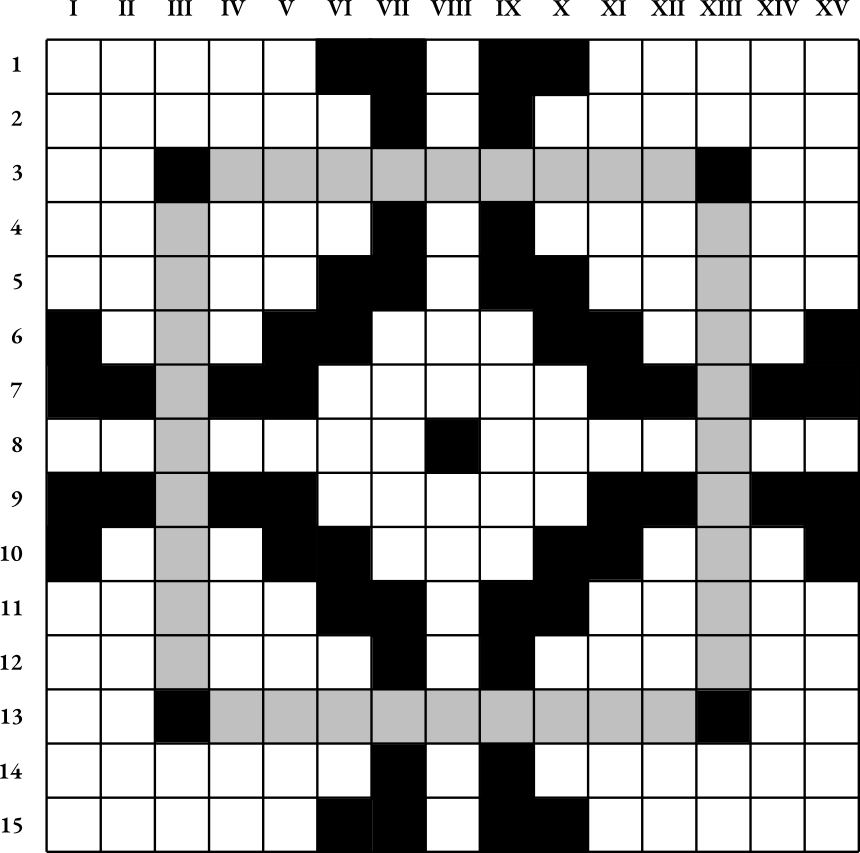
\includegraphics[width=\textwidth]{puzzle}
\end{center}

\pagebreak[2]

{\scshape\large\bfseries Across.}

\def\arraystretch{2.5}
	
\begin{longtable} {c p{0.8\linewidth}} 
\textsc{i}.1. & \makecell[l]{Foolish or wise, yet one remains alone,\\'Twixt Strength and Justice on a heavenly throne.}\\
\textsc{xi}.1. & \makecell[l]{O to what ears the chink of gold was sweet;\\
The greed for treasure brought him but defeat.}\\
\end{longtable}

»That's a hint to us,« said Lord~Peter.

\begin{longtable} {c p{0.8\linewidth}} 
\textsc{i}.2. &  \makecell[l]{One drop of vinegar to two of oil\\
Dresses this curly head sprung from the soil.}\\
\textsc{x}.2. &  \makecell[l]{Nothing itself, it needs but little more\\
To be that nothingness the Preacher saw.}\\
\textsc{i}.3. &  \makecell[l]{Dusty though my fellows be,\\
We are a kingly company.}\\
\textsc{iv}.3. &  \makecell[l]{Have your own will, though here, I hold,\\
The new is not a patch upon the old.}\\
\textsc{xiv}.3. &  \makecell[l]{Any loud cry would do as well,\\
Or so the poet's verses tell.}\\
\textsc{i}.4. & \makecell[l]{ This is the most unkindest cut of all,\\
Except your skill be mathematical.}\\
\textsc{x}.4. &  \makecell[l]{Little and hid from mortal sight,\\
I darkly work to make all light.}\\
\textsc{i}.5. &  \makecell[l]{The need for this (like that it's cut off short)\\
The building of a tower to humans taught.}\\
\textsc{xi}.5. & \makecell[l]{ »More than a mind discloses and more than men believe«\\
(A definition by a man whom Pussyfoot doth grieve).}\\
\textsc{ii}.6. &  \makecell[l]{Backward observe her turn her way,\\
The way of wisdom, wise men say.}\\
\textsc{vii}.6. &  \makecell[l]{Grew long ago by river's edge\\
Where grows to-day the common sedge.}\\
\textsc{xii}.6. &  \makecell[l]{One of three by which, they say,\\
You'll know the Cornishmen alway.}\\
\textsc{vi}.7. &  \makecell[l]{Blow upon blow; five more the vanquished Roman shows;\\
And if the foot slip one, on crippled feet one goes.}\\
\textsc{i}.8. &  \makecell[l]{By this Jew's work the whole we find,\\
in a glass clearly, darkly in the mind.}\\
\textsc{ix}.8. &  \makecell[l]{Little by little see it grow\\
Till cut off short by hammer-blow.}\\
\textsc{vi}.9. &  \makecell[l]{Watch him go, heel and toe,\\
Across the wide Karroo!}\\
\textsc{ii}.10. &  \makecell[l]{In expectation to be rich\\
Here you reach the highest pitch.}\\
\textsc{vii}.10. &  \makecell[l]{Of this, concerning nothing, much—\\
Too often do we hear of such!}\\
\textsc{xii}.10. &  \makecell[l]{O'er land and sea, passing on deadly wings,\\
Pain to the strong, to weaklings death it brings.}\\
\textsc{i}.11. &  \makecell[l]{Requests like these, however long they be,\\
Stop just too soon for common courtesy.}\\
\textsc{xi}.11. &  \makecell[l]{Cæsar, the living dead salute thee here,\\
Facing for thy delight tooth, claw, and spear.}\\
\textsc{i}.12. &  \makecell[l]{One word had served, but he in ranting vein\\
»Lend me your ears« must mouth o'er Cæsar slain.}\\
\textsc{x}.12. &  \makecell[l]{Helical circumvolution\\
Adumbrates correct solution.}\\
\textsc{i}.13. &  \makecell[l]{One that works for Irish men\\
Both by word and deed and pen.}\\
\end{longtable}

»That's an easy one,« said Miss Marryat.

\begin{longtable} {c p{0.8\linewidth}} 
\textsc{iv}.13. &  \makecell[l]{Seven out of twelve this number makes complete\\
As the sun journeys on from seat to seat.}\\
\textsc{xiv}.13. &  \makecell[l]{My brothers play with planets; Cicero,\\
Master of words, my master is below.}\\
\textsc{i}.14. &  \makecell[l]{Free of her jesses let the falcon fly,\\
With sight undimmed into the azure sky.}\\
\textsc{x}.14. &  \makecell[l]{And so you dine with Borgia? Let me lend\\
You this as a precaution, my poor friend.}\\
\textsc{i}.15. &  \makecell[l]{Friendship carried to excess\\
Got him in a horrid mess.}\\
\textsc{xi}.15. &  \makecell[l]{Smooth and elastic and, I guess,\\
The dearest treasure you possess.}\\
\end{longtable}

\pagebreak[2]

{\scshape\large\bfseries Down.}

\begin{longtable} {c p{0.8\linewidth}} 
1.\textsc{i.} &  \makecell[l]{If step by step the Steppes you wander through\\
Many of those in this, of these in those you'll view.}\\
\end{longtable}

»Bunter,« said Lord~Peter, »bring me a whisky-and-soda!«

\begin{longtable} {c p{0.8\linewidth}}
11.\textsc{i.} &  \makecell[l]{If me without my head you do,\\
Then generously my head renew,\\
Or put it to my hinder end—\\
Your cheer it shall nor mar nor mend.}\\
1.\textsc{ii.} &  \makecell[l]{Quietly, quietly, 'twixt edge and edge,\\
Do this unto the thin end of the wedge.}\\
10.\textsc{ii.} &  \makecell[l]{»Something that hath a reference to my state?«\\
Just as you like, it shall be written straight.}\\
1.\textsc{iii.} & \makecell[l]{ When all is read, then give the world its due,\\
And never need the world read this of you.}\\
\end{longtable}


»That's a comfort,« said Lady~Mary. »It shows we're on the right lines.«

\begin{longtable} {c p{0.8\linewidth}} 
4.\textsc{iii.} &  \makecell[l]{Sing Nunc Dimittis and Magnificat—\\
But look a little farther back than that.}\\
14.\textsc{iii.} &  \makecell[l]{Here in brief epitome\\
Attribute of royalty.}\\
1.\textsc{iv.} &  \makecell[l]{Lo! at a glance\\
The Spanish gipsy and her dance.}\\
10.\textsc{iv.} &  \makecell[l]{Bring me skin and a needle or a stick—\\
A needle does it slowly, a stick does it quick.}\\
1.\textsc{v.} &  \makecell[l]{It was a brazen business when\\
King Phalaris made these for men.}\\
11.\textsc{v.} &  \makecell[l]{This king (of whom not much is known),\\
By Heaven's mercy was o'erthrown.}\\
2.\textsc{vi.} &  \makecell[l]{»Bid [Greek:'on kai mê 'on] farewell?« Nay, in this\\
The sterner Roman stands by that which is.}\\
7.\textsc{vi.} &  \makecell[l]{This the termination is\\
Of many minds' activities.}\\
12.\textsc{vi.} &  \makecell[l]{I mingle on Norwegian shore,\\
With ebbing water's backward roar.}\\
6.\textsc{vii.} &  \makecell[l]{I stand, a ladder to renown,\\
Set 'twixt the stars and Milan town.}\\
1.\textsc{viii.} &  \makecell[l]{Highest and lowliest both to me lay claim,\\
The little hyssop and the king of fame.}\\
\end{longtable}


»That makes that point about the squares clear,« said Mary.

»I think it's even more significant,« said her brother.

\begin{longtable} {c p{0.8\linewidth}} 
9.\textsc{viii.} &  \makecell[l]{This sensible old man refused to tread\\
The path to Hades in a youngster's stead.}\\
6.\textsc{ix.} &  \makecell[l]{Long since, at Nature's call, they let it drop,\\
Thoughtlessly thoughtful for our next year's crop.}\\
2.\textsc{x.} &  \makecell[l]{To smallest words great speakers greatness give;\\
Here Rome propounded her alternative.}\\
7.\textsc{x.} &  \makecell[l]{We heap up many with toil and trouble,\\
And find that the whole of our gain is a bubble.}\\
12.\textsc{x.} &  \makecell[l]{Add it among the hidden things—\\
A fishy tale to light it brings.}\\
1.\textsc{xi.} &  \makecell[l]{»Lions,« said a Gallic critic, »are not these.«\\
Benevolent souls—they'd make your heart's blood freeze.}\\
11.\textsc{xi.} &  \makecell[l]{An epithet for husky fellows,\\
That stand, all robed in greens and yellows.}\\
1.\textsc{xii.} &  \makecell[l]{Whole without holes behold me here,\\
My meaning should be wholly clear.}\\
10.\textsc{xii.} &  \makecell[l]{Running all around, never setting foot to floor,\\
If there isn't one in this room, there may be one next door.}\\
1.\textsc{xiii.} &  \makecell[l]{Ye gods! think also of that goddess' name\\
Whose might two hours on end the mob proclaim.}\\
4.\textsc{xiii.} &  \makecell[l]{The Priest uplifts his voice on high,\\
The choristers make their reply.}\\
14.\textsc{xiii.} &  \makecell[l]{When you've guessed it, with one voice\\
You'll say it was a golden choice.}\\
1.\textsc{xiv.} &  \makecell[l]{Shall learning die amid a war's alarms?\\
I, at my birth, was clasped in iron arms.}\\
10.\textsc{xiv.} &  \makecell[l]{At sunset see the labourer now\\
Loose all his oxen from the plough.}\\
1.\textsc{xv.} &  \makecell[l]{Without a miracle it cannot be—\\
At this point, Solver, bid him pray for thee!}\\[.3cm] 
11.\textsc{xv.} &  \makecell[l]{Two thousand years ago and more\\
(Just as we do to-day),\\
The Romans saw these distant lights—\\
But, oh! how hard the way!}
\end{longtable}

\divider
The most remarkable part of the search—or so Lord~Peter thought—was its effect on Miss Marryat. At first she hovered disconsolately on the margin, aching with wounded dignity, yet ashamed to dissociate herself from people who were toiling so hard and so cheerfully in her cause.

»I think that's so-and-so,« Mary would say hopefully.

And her brother would reply enthusiastically, »Holed it in one, old lady. Good for you! We've got it this time, Miss Marryat«—and explain it.

And Hannah Marryat would say with a snort:

»That's just the childish kind of joke Uncle Meleager would make.«

Gradually, however, the fascination of seeing the squares fit together caught her, and, when the first word appeared which showed that the searchers were definitely on the right track, she lay down flat on the floor and peered over Lord~Peter's shoulder as he grovelled below, writing letters in charcoal, rubbing them out with his handkerchief and mopping his heated face, till the Moor of Venice had nothing on him in the matter of blackness. Once, half scornfully, half timidly, she made a suggestion; twice, she made a suggestion; the third time she had an inspiration. The next minute she was down in the mêlée, crawling over the tiles flushed and excited, wiping important letters out with her knees as fast as Peter could write them in, poring over the pages of Roget, her eyes gleaming under her tumbled black fringe.

Hurried meals of cold meat and tea sustained the exhausted party, and towards sunset Peter, with a shout of triumph, added the last letter to the square.

They crawled out and looked at it.

»All the words can't be clues,« said Mary. »I think it must be just those four.«

»Yes, undoubtedly. It's quite clear. We've only got to look it up. Where's a Bible?«

Miss Marryat hunted it out from the pile of reference books. »But that isn't the name of a Bible book,« she said. »It's those things they have at evening service.«

»That's all you know,« said Lord~Peter. »I was brought up religious, I was. It's Vulgate, that's what that is. You're quite right, of course, but, as Uncle Meleager says, we must »look a little farther back than that.« Here you are. Now, then.«

»But it doesn't say what chapter.«

»So it doesn't. I mean, nor it does.«

»And, anyhow, all the chapters are too short.«

»Damn! Oh! Here, suppose we just count right on from the beginning—one, two, three\longdash«

»Seventeen in chapter one, eighteen, nineteen—this must be it.«

Two fair heads and one dark one peered excitedly at the small print, Bunter hovering decorously on the outskirts.

»O my dove, that art in the clefts of the rock, in the covert of the steep place.«

»Oh, dear!« said Mary, disappointed, »that does sound rather hopeless. Are you sure you've counted right? It might mean anything.«

Lord~Peter scratched his head.

»This is a bit of a blow,« he said. »I don't like Uncle Meleager half as much as I did. Old beast!«

»After all our work!« moaned Mary.

»It must be right,« cried Miss Marryat. »Perhaps there's some kind of an anagram in it. We can't give up now!«

»Bravo!« said Lord~Peter. »That's the spirit. 'Fraid we're in for another outburst of frivolity, Miss Marryat.«

»Well, it's been great fun,« said Hannah Marryat.

»If you will excuse me,« began the deferential voice of Bunter.

»I'd forgotten you, Bunter,« said his lordship. »Of course you can put us right—you always can. Where have we gone wrong?«

»I was about to observe, my lord, that the words you mention do not appear to agree with my recollection of the passage in question. In my mother's Bible, my lord, it ran, I fancy, somewhat differently.«

Lord~Peter closed the volume and looked at the back of it.

»Naturally,« he said, »you are right again, of course. This is a Revised Version. It's your fault, Miss Marryat. You would have a Revised Version. But can we imagine Uncle Meleager with one? No. Bring me Uncle Meleager's Bible.«

»Come and look in the library,« cried Miss Marryat, snatching him by the hand and running. »Don't be so dreadfully calm.«

On the centre of the library table lay a huge and venerable Bible—reverend in age and tooled leather binding. Lord~Peter's hands caressed it, for a noble old book was like a song to his soul. Sobered by its beauty, they turned the yellow pages over:

»In the clefts of the rocks, in the secret places of the stairs.«

»Miss Marryat,« said his lordship, »if your Uncle's will is not concealed in the staircase, then—well, all I can say is, he's played a rotten trick on us,« he concluded lamely.

»Shall we try the main staircase, or the little one up to the porch?«

»Oh, the main one, I think. I hope it won't mean pulling it down. No. Somebody would have noticed if Uncle Meleager had done anything drastic in that way. It's probably quite a simple hiding-place. Wait a minute. Let's ask the housekeeper.«

Mrs~Meakers was called, and perfectly remembered that about nine months previously Mr~Finch had pointed out to her a »kind of a crack like« on the under surface of the staircase, and had had a man in to fill it up. Certainly, she could point out the exact place. There was the mark of the plaster filling quite clear.

»Hurray!« cried Lord~Peter. »Bunter—a chisel or something. Uncle Meleager, Uncle Meleager, we've got you! Miss Marryat, I think yours should be the hand to strike the blow. It's your staircase, you know—at least, if we find the will, so if any destruction has to be done it's up to you.«

Breathless they stood round, while with a few blows the new plaster flaked off, disclosing a wide chink in the stonework. Hannah Marryat flung down hammer and chisel and groped in the gap.

»There's something,« she gasped. »Lift me up; I can't reach. Oh, it is! it is! it is it!« And she withdrew her hand, grasping a long, sealed envelope, bearing the superscription:

\begin{center}\scshape\large
Positively the \textbf{LAST} Will and Testament of Meleager Finch.
\end{center}

Miss Marryat gave a yodel of joy and flung her arms round Lord~Peter's neck.

Mary executed a joy-dance. »I'll tell the world,« she proclaimed.

»Come and tell mother!« cried Miss Marryat.

Mr~Bunter interposed,

»Your lordship will excuse me,« he said firmly, »but your lordship's face is all over charcoal.«

»Black but comely,« said Lord~Peter, »but I submit to your reproof. How clever we've all been. How topping everything is. How rich you are going to be. How late it is and how hungry I am. Yes, Bunter, I will wash my face. Is there anything else I can do for anybody while I feel in the mood?«

»If your lordship would be so kind,« said Mr~Bunter, producing a small paper from his pocket, »I should be grateful if you could favour me with a South African quadruped in six letters, beginning with Q\@.«
\vfill
\textsc{Note}.—The solution of the cross-word will be found at the end of the book.